\documentclass{csse4400}

% \teachermodetrue

\usepackage{float}

\usepackage{languages}

\title{TLDR of Databases in Applications}
\author{Brae Webb \& Evan Hughes}

\date{\week{2}}
\begin{document}

\maketitle

\begin{figure}[h]
  \href{https://www.oreilly.com/library/view/designing-data-intensive-applications/9781491903063/ch02.html}{
    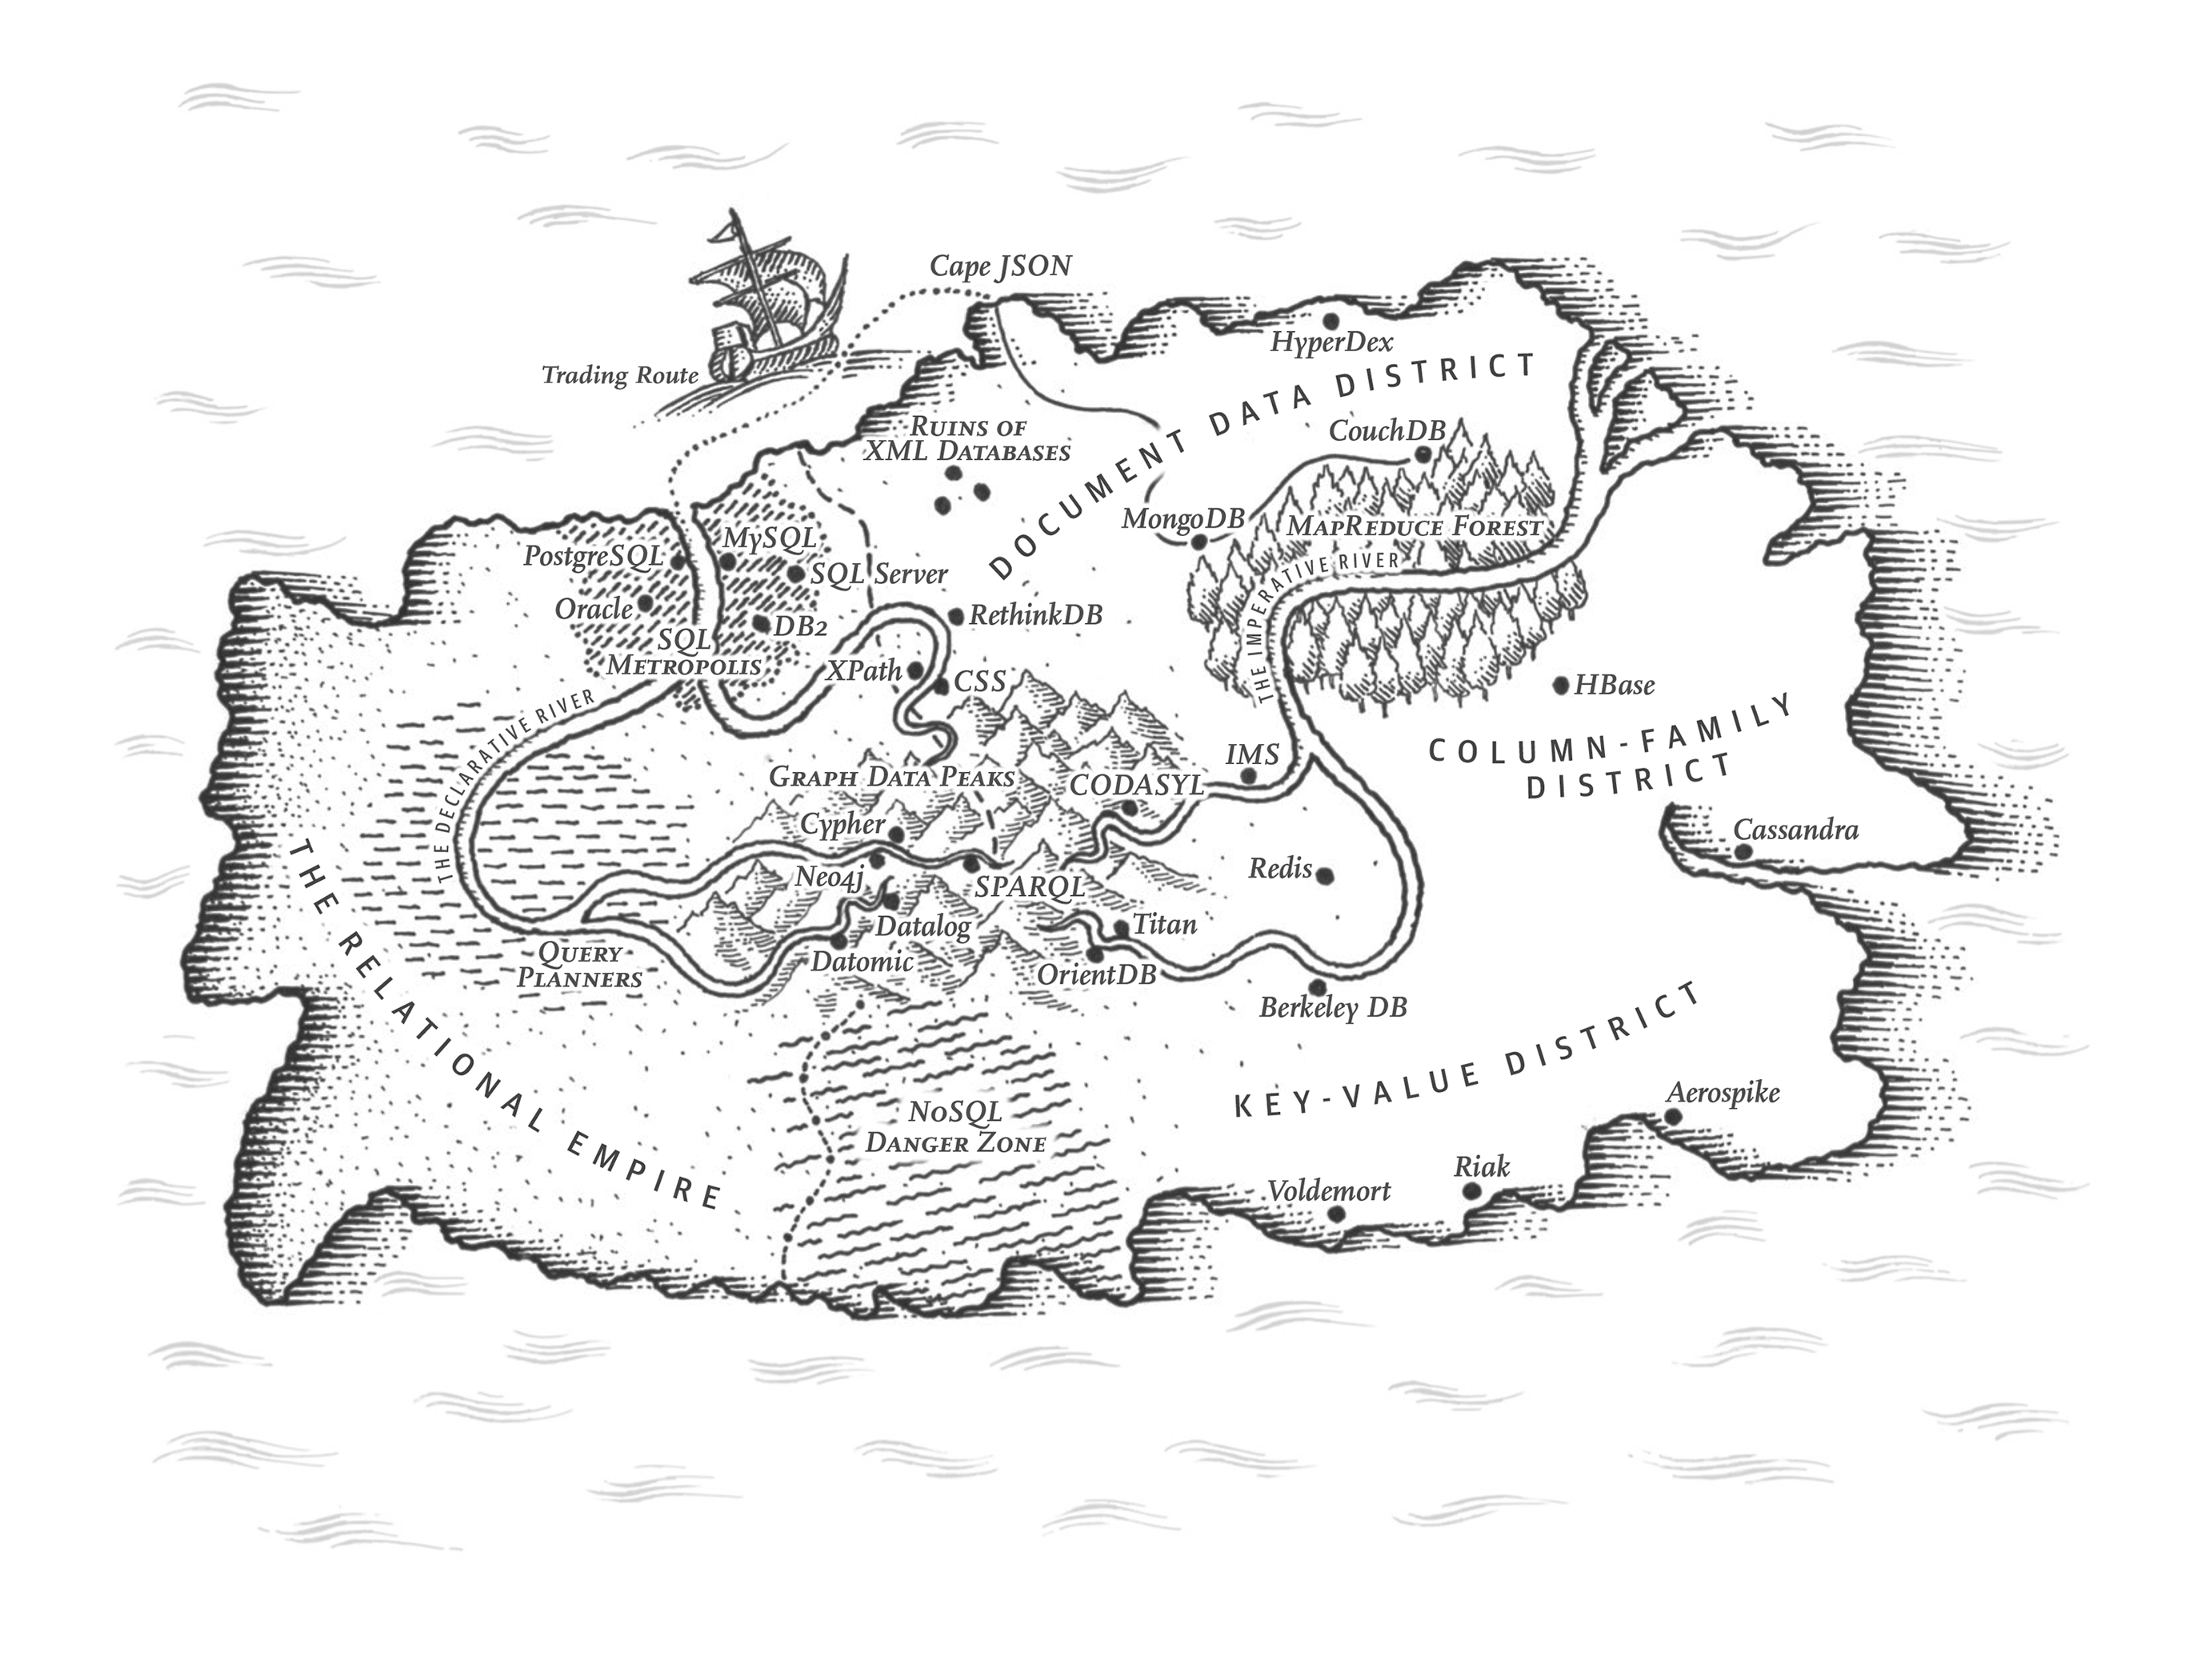
\includegraphics[width=\textwidth]{images/databases}
  }
\caption{A map of data storage techniques from Designing Data-Intensive Applications \cite{data-intensive}.}
\end{figure}

\section{This Week}
This week our goal is to:
\begin{itemize}
  \item explore the various techniques developers use to store data;
  \item investigate the storage options implementing these techniques on the AWS platform;
  \item upgrade our todo application to use a relational database;
\end{itemize}

\section{Databases and Data Models}
Unfortunately, to build interesting software we often need to store and use data.
The storage of data introduces a number of challenges when designing, creating, and maintaining our software.
However, not all data storage techniques are created equal;
the choice of data storage model can have a profound impact on our software's complexity and maintainability.
In this practical, we want to take a superficial exploration of our island of data storage models.
For a more in-depth treatment of data storage models that is outside the scope of this course,
see Chapter 2 of the \textit{Designing Data-Intensive Applications} book \cite{data-intensive}.


\teacher{
  Discuss the following different storage technologies and mention some use cases of when you would choose each one.
  Discuss some popular implementations of each.\\

  Aim for no more than 30 minutes of discussion.
}

\subsection{Relational Storage}

Relational databases what have been exposed to the most in your University career --- think MySQL, Postgres, Oracle DB, etc.
This type of database is good at modelling the real world which is often a highly connected environment.
% The data model that is suggested for this type of storage is a normalised approach where data duplication should be reduced.

Some popular offerings are below:

\begin{itemize}
  \item MySQL/MariaDB [ Amazon RDS / Amazon Aurora ].
  \item Postgres [ Amazon RDS / Amazon Aurora ].
\end{itemize}

The AWS offerings of these services come in two different types, we have the traditional approach of
server capacity ( x cores, y ram ) and we have a server-less approach.
The server-less approach is a more dynamic
database that can scale to large amounts of load when needed though at a cost per request.

  \subsubsection{ORM}
  Object Relational Mapping (ORM) is a fairly common tool for programmers to use to make developing with databases smoother.
  One fairly prevalent example of this is SQLAlchemy which is a very widely used 
  database abstraction for python.
  SQLAlchemy allows us to move to a higher level of abstraction than SQL queries and perform database actions using standard python code.

  The benefits of ORMs are the ability to model database objects in our existing programming language instead of having large blocks of SQL text within our source code.
  The disadvantages come in when we need to do specific SQL work or where the abstractions cost is greater than the benefits.

\subsection{Wide-Column Storage}

\teacher{
  Examples of big apps that depend on this technology is Netflix \url{https://netflixtechblog.com/netflixs-viewing-data-how-we-know-where-you-are-in-house-of-cards-608dd61077da}.
}

Wide-Column databases are a form of NoSQL or non-relational data stores.
In these data stores the data model design 
is focused more on having efficient queries at the cost of data duplication.
A warning to the reader that these models
are not flexible after creation, it is much easier to answer a new use case in a relational model.

  \begin{itemize}
    \item Apache Cassandra [ Amazon Keyspaces for Cassandra ].
    \item Apache HBase.
  \end{itemize}

\subsection{Key-Value Storage}

Key-Value stores are very popular for cache or remote config use cases, some of the most notable are Redis and Memcached.
These stores allow efficient lookup of values via keys and are usually stored in-memory.

\begin{itemize}
  \item Redis [ Amazon ElastiCache for Redis ].
  \item Memcached [ Amazon ElastiCache for Memcached].
  \item Amazon DynamoDB.
  \item Amazon MemoryDB for Redis.
\end{itemize}

\subsection{Time Series Storage}

\teacher{
  Something to mention here is that relations are usually not utilised between tables in time series databases.
}

Time series databases are highly focused storage which is tailored to retrieving results by timestamp ranges.
Many implementations also take advantage of the data model to allow efficient rollover of data and partitioning.
One of the most popular time series databases is Prometheus which is used to store monitoring metrics.

\begin{itemize}
  \item Amazon Timestream.
  \item TimescaleDB ( Postgres + Addon ).
  \item Prometheus.
  \item InfluxDB.
\end{itemize}

\subsection{Document Storage}

Document databases are a subset of NoSQL databases with a focus on a flexible data model.
MongoDB for instance allows the user to store JSON documents and perform queries on those documents.
One advantage of document databases is that they match a programmers existing mental model of storing data in formats such as JSON.

\begin{itemize}
  \item MongoDB.
  \item Apache CouchDB.
  \item Amazon DocumentDB.
  \item Amazon DynamoDB.
\end{itemize}

\subsection{Graph Storage}

\teacher{
  If you havnt experienced graph databases, a good usecase is ``recommendation systems'',
  which use the connected nature of items to figure out what to suggest to a person.Another example is the \url{https://neo4j.com/blog/analyzing-panama-papers-neo4j/}
  Panama Papers.
}

Graph Databases are relational storage with a few enhancements to allow fast neighbour look-ups.
These databases also allow the implementation of graph algorithms to query data.

\begin{itemize}
  \item Amazon Neptune.
  \item Neo4J.
  \item Janus Graph.
\end{itemize}

\section{Enhancing the Todo App with Storage}

Last week we created a simple web server that can listen on a port and respond to HTTP requests. The endpoints that we created are all stubs the return a simple JSON response. This week we will be adding a database to our application to store the todo items.

\subsection{Creating a Practical Repository}
Navigate to the GitHub Classroom link provided by your tutor.
You should see a list of practicals, click on the week one practical.
This will create a new repository for you in the course organisation.
You can now clone this repository to your local machine or work directly in the browser with GitHub codespaces.

\info{
  If using Github CodeSpaces the environment will be pre-installed with the libraries you used last week. You will still need to follow on with the instructions below to install the database libraries.
}

\subsection{Installing the Database Dependencies}

We will be using a python library called SQLAlchemy to interact with our database. This library abstracts the low level SQL queries away from us and allows us to interact with the database using python objects. We will be using SQLAlchemy using a packaged called Flask-SQLAlchemy which is a wrapper around SQLAlchemy that is designed to work with Flask our WebServer library.

\begin{code}[language=bash,numbers=none]{}
  >> pipenv install flask-sqlalchemy
\end{code}

\subsection{Creating the Database Models}

We will be using a database called SQLite for this practical. SQLite is a file based database which is very easy to setup and use. It is also a good choice for development as it can be blown away by simply deleting a file or by residing in memory.

Now that our dependencies are installed, lets start by navigating to our new cloned practical folder and creating a new folder called models. Inside this folder we will create a new file called todo.py and a new file called \texttt{\_\_init\_\_.py}.

Inside the \texttt{\_\_init\_\_.py} file we will add the following code:

\begin{code}[language=python,numbers=none]{}
  from flask_sqlalchemy import SQLAlchemy

  db = SQLAlchemy()
\end{code}

All this file does is setup a new SQLAlchemy object which we will use to interact with our database. In the \texttt{todo.py} file we will add the following code:

\begin{code}[language=python,numbers=none]{}
  import datetime
  from models import db

  class Todo(db.Model):
      id = db.Column(db.Integer, primary_key=True)
      title = db.Column(db.String(80), nullable=False)
      description = db.Column(db.String(120), nullable=True)
      completed = db.Column(db.Boolean, nullable=False, default=False)
      deadline_at = db.Column(db.DateTime, nullable=True)
      created_at = db.Column(db.DateTime, nullable=False, default=datetime.datetime.utcnow)
      updated_at = db.Column(db.DateTime, nullable=False, default=datetime.datetime.utcnow, onupdate=datetime.datetime.utcnow)

      def to_dict(self):
          return {
              'id': self.id,
              'title': self.title,
              'description': self.description,
              'completed': self.completed,
              'deadline_at': self.deadline_at.isoformat() if self.deadline_at else None,
              'created_at': self.created_at.isoformat() if self.created_at else None,
              'updated_at': self.updated_at.isoformat() if self.updated_at else None,
          }

      def __repr__(self):
          return f'<Todo {self.title}>'
\end{code}

The above code is doing a lot of the heavy lifting for us in our database table generation so lets walk through and see what some of the key lines are doing.

\begin{code}[language=python,numbers=none]{}
  class Todo(db.Model):
\end{code}

This line is defining a new class called Todo which inherits from the db.Model class. This class will be used to represent our todo items in our database.

\begin{code}[language=python,numbers=none]{}
  id = db.Column(db.Integer, primary_key=True)
\end{code}

This line is defining a new column in our database table called id. The column type is an integer and it is the primary key for the table. As we insert more items into our database, the id will be automatically incremented for us.

\begin{code}[language=python,numbers=none]{}
  title = db.Column(db.String(80), nullable=False)
\end{code}

This line is defining a new column in our database table called title. The column type is a string with a maximum length of 80 characters. The nullable parameter is set to false which means that this column cannot be null. Essentially this is a required field.

\begin{code}[language=python,numbers=none]{}
  description = db.Column(db.String(120), nullable=True)
\end{code}

This line is defining a new column in our database table called description. The column type is a string with a maximum length of 120 characters. The nullable parameter is set to true which means that this column can be null. Essentially this is an optional field.

\begin{code}[language=python,numbers=none]{}
  completed = db.Column(db.Boolean, nullable=False, default=False)
\end{code}

This line is defining a new column in our database table called completed. The column type is a boolean which can be either true or false. The nullable parameter is set to false which means that this column cannot be null. The default parameter is set to false which means that if no value is provided for this column, it will default to false.

\begin{code}[language=python,numbers=none]{}
  deadline_at = db.Column(db.DateTime, nullable=True)
\end{code}

This line is defining a new column in our database table called \texttt{deadline\_at}. The column type is a datetime so we can represent the time when the todo is due.

\begin{code}[language=python,numbers=none]{}
  created_at = db.Column(db.DateTime, nullable=False, default=datetime.datetime.utcnow)
\end{code}

This line is defining a new column in our database table called \texttt{created\_at}. The column type is a datetime so we can represent the time when the todo was created. The extra addition here is that the default parameter is a reference to a function called \texttt{utcnow} which will automatically set the value of this column to the current time when the todo is created.

\begin{code}[language=python,numbers=none]{}
  updated_at = db.Column(db.DateTime, nullable=False, default=datetime.datetime.utcnow, onupdate=datetime.datetime.utcnow)
\end{code}

This line is defining a new column in our database table called \texttt{updated\_at}. The column type is a datetime so we can represent the time when the todo was last updated. The extra addition onupdate parameter is a reference to a function called \texttt{utcnow} which will automatically set the value of this column to the current time when the todo is updated.

\begin{code}[language=python,numbers=none]{}
  def to_dict(self):
      return {
          'id': self.id,
          'title': self.title,
          'description': self.description,
          'completed': self.completed,
          'deadline_at': self.deadline_at.isoformat() if self.deadline_at else None,
          'created_at': self.created_at.isoformat() if self.created_at else None,
          'updated_at': self.updated_at.isoformat() if self.updated_at else None,
      }
\end{code}

This is a method on our Todo class which will return a dictionary representation of the todo item. This is useful for when we want to return the todo item as JSON in our API as it deals with converting the datetime objects into a particular string format.

\begin{code}[language=python,numbers=none]{}
  def __repr__(self):
      return f'<Todo {self.id} - {self.title}>'
\end{code}

This is a method on our Todo class which will return a string representation of the todo item. This is useful for debugging purposes as it will print out the ID and title of the Todo.

\subsection{Configuring the Database}

Now that we have defined our database table, we need to configure our application to use the database. Open the \texttt{todo/\_\_init\_\_.py} file and change the code to the following:

\begin{code}[language=python,numbers=none]{}
  from flask import Flask
  from flask_sqlalchemy import SQLAlchemy
  from flask_migrate import Migrate

  def create_app():
      app = Flask(__name__)

      app.config['SQLALCHEMY_DATABASE_URI'] = "sqlite:///db.sqlite"

      # Load the models
      from todo.models import db
      db.init_app(app)

      # Create the database tables
      db.create_all()

      # Register the blueprints
      from todo.views.routes import api
      app.register_blueprint(api)

      return app

\end{code}

This will load the models we defined in the previous section and create the database tables for us. We also need to tell our application where the database is located. We can do this by setting the \texttt{SQLALCHEMY\_DATABASE\_URI} config variable. In this case we are using a SQLite database which is a file based database. We can set the location of the database by setting the \texttt{SQLALCHEMY\_DATABASE\_URI} config variable to the path of the database file. In this case we are using a relative path to the \texttt{db.sqlite} file in the root of our project.

If we run our application now, we will see that the database file has been created for us.

\todo{
  Add a screenshot of the database file being created.
}

\subsection{Inspecting the Database}

We can use the \texttt{sqlite3} command line tool to inspect the database. Open a terminal and navigate to the root of your project. Then run the following command:

\begin{code}[language=bash,numbers=none]{}
  sqlite3 db.sqlite
\end{code}

This will open the SQLite command line tool and connect to the database file. We can then run the following command to see the tables in our database:

\begin{code}[language=sql,numbers=none]{}
  .tables
\end{code}

This will show us the tables in our database. We can then run the following command to see the columns in our table:

\begin{code}[language=sql,numbers=none]{}
  .schema todos
\end{code}

This will show us the columns in our table. We can then run the following command to see the data in our table:

\begin{code}[language=sql,numbers=none]{}
  SELECT * FROM todos;
\end{code}

This will show us the data in our table. We can then run the following command to exit the SQLite command line tool:

\begin{code}[language=sql,numbers=none]{}
  .exit
\end{code}

You may have noticed that our table is called todos and not todo. This is because SQLAlchemy will automatically pluralise the name of the table for us. This is a common behaviour you will see many database libraries.


\subsection{Using the Database}

Now that we have a database intergrated into our application, lets modify our endpoints to take advantage of it. 

Open the \texttt{todo/views/routes.py} file and add the following imports to the top of the file:

\begin{code}[language=python,numbers=none]{}
  from todo.models import db
  from todo.models.todo import Todo
\end{code}

Open the \texttt{todo/views/routes.py} file and change the \texttt{get\_todos} endpoint to the following:

\begin{code}[language=python,numbers=none]{}
  @api.route('/todos', methods=['GET'])
  def get_todos():
      todos = Todo.query.all()
      return jsonify([todo.to_dict() for todo in todos])
\end{code}

This will query the database for all the todos and return them as JSON. We can then change the \texttt{get\_todo} endpoint to the following:

\begin{code}[language=python,numbers=none]{}
  @api.route('/todos/<int:id>', methods=['GET'])
  def get_todo(id):
      todo = Todo.query.get(id)
      if todo is None:
          return make_response(jsonify({'error': 'Todo not found'}, 404)
      return make_response(jsonify(todo.to_dict()))
\end{code}

So we have upgraded these endpoints to use the database. Lets test that our application is still functioning correctly. Restart your webserver and navigate to the \texttt{/todos} endpoint. You should see the following JSON response:

\begin{code}[language=json,numbers=none]{}
  []
\end{code}

Of course our API does not have any todo items in it yet. Lets add some todo items to our database. Open the \texttt{todo/views/routes.py} file and change the \texttt{create\_todo} endpoint to the following:

\begin{code}[language=python,numbers=none]{}
  @api.route('/todos', methods=['POST'])
  def create_todo():
      todo = Todo(
          title=request.json.get('title'),
          description=request.json.get('description'),
          completed=request.json.get('completed', False),
          deadline_at=request.json.get('deadline_at')
      )
      db.session.add(todo)
      db.session.commit()
      return make_response(jsonify(todo.to_dict()), 201)
\end{code}

This endpoint now lets us create a todo item in the database. Lets test this endpoint by going to our endpoints.http and running the POST request. You should see the following response:

\begin{code}[language=json,numbers=none]{}
  {
    "id": 1,
    "title": "Test Todo",
    "description": "This is a test todo",
    "completed": false,
    "deadline_at": null,
    "created_at": "2023-02-27T12:00:00.000000Z",
    "updated_at": "2023-02-27T12:00:00.000000Z"
  }
\end{code}

Now if we go to our \texttt{/todos} endpoint we should see the todo item we just created. You should see the following response:

\begin{code}[language=json,numbers=none]{}
  [
    {
      "id": 1,
      "title": "Test Todo",
      "description": "This is a test todo",
      "completed": false,
      "deadline_at": null,
      "created_at": "2023-02-27T12:00:00.000000Z",
      "updated_at": "2023-02-27T12:00:00.000000Z"
    }
  ]
\end{code}

Now lets add the remaining endpoints. Open the \texttt{todo/views/routes.py} file and change the \texttt{update\_todo} endpoint to the following:

\begin{code}[language=python,numbers=none]{}
  @api.route('/todos/<int:id>', methods=['PUT'])
  def update_todo(id):
      todo = Todo.query.get(id)
      if todo is None:
          return make_response(jsonify({'error': 'Todo not found'}, 404)
      todo.title = request.json.get('title', todo.title)
      todo.description = request.json.get('description', todo.description)
      todo.completed = request.json.get('completed', todo.completed)
      todo.deadline_at = request.json.get('deadline_at', todo.deadline_at)
      db.session.commit()
      return make_response(jsonify(todo.to_dict()))

\end{code}

This endpoint will update a todo item in the database. Lets test this endpoint by going to our endpoints.http and running the PUT request. You should see the following response:

\begin{code}[language=json,numbers=none]{}
  {
    "id": 1,
    "title": "Updated Test Todo",
    "description": "This is an updated test todo",
    "completed": false,
    "deadline_at": null,
    "created_at": "2023-02-27T12:00:00.000000Z",
    "updated_at": "2023-02-27T12:00:00.000000Z"
  }

\end{code}

The delete endpoint we will write is very similar to the update endpoint. Open the \texttt{todo/views/routes.py} file and change the \texttt{delete\_todo} endpoint to the following:

\begin{code}[language=python,numbers=none]{}
  @api.route('/todos/<int:id>', methods=['DELETE'])
  def delete_todo(id):
      todo = Todo.query.get(id)
      if todo is None:
          return make_response(jsonify(), 200)

      db.session.delete(todo)
      db.session.commit()
      return make_response(jsonify({'message': 'Todo deleted'}), 200)

\end{code}

We now have a set of endpoints that can perform the CRUD operations of our API but some functionality is missing. We are gonna add that functionality after writing some tests to help us do \textbf{Test Driven Development}.

\section{Testing the API}

\subsection{Setting up the testing environment}

In the root folder of this practical make a \texttt{tests} folder. Inside the \texttt{tests} folder create a \texttt{base.py} file. Inside the \texttt{base.py} file add the following code:

\begin{code}[language=python,numbers=none]{}
  from todo import create_app
  import unittest
  
  
  class TodoTest(unittest.TestCase):
      def setUp(self):
          self.app = create_app(config_overrides={
              'SQLALCHEMY_DATABASE_URI': 'sqlite:///:memory:',
              'TESTING': True
          })
  
          with self.app.app_context():
              from todo.models import db
              db.create_all()
              db.session.commit()
          
          self.client = self.app.test_client()
  
      def assertTodoPartialEqual(self, todo: dict, expected: dict):
          for key, value in expected.items():
              self.assertEqual(todo[key], value)
\end{code}


This base class is what we will use to help setup our tests and provide some helper methods. We will be using the \texttt{unittest} library to write our tests. The \texttt{setUp} method is called before each test and is used to setup the testing environment. The \texttt{assertTodoPartialEqual} method is a helper method that we will use to compare the todo items we get from the API with the todo items we expect to get from the API.

As you can see we have a slight modification to the \texttt{create\_app} function. We are passing in a dictionary of config overrides. This allows us to override the config values for the testing environment. We are overriding the \texttt{SQLALCHEMY\_DATABASE\_URI} to use an in memory database. This means that the database will be created in memory and will be destroyed when the tests are finished. We are also overriding the \texttt{TESTING} config value to be true. This will allow us to use the \texttt{test\_client} method on our app to make requests to our API.

\subsection{Prepping the config for testing}

Open the \texttt{todo/\_\_init\_\_.py} file and adjust the \texttt{create\_app} function to the following:

\begin{code}[language=python,numbers=none]{}
  def create_app(config_overrides=None):
      app = Flask(__name__)

      app.config['SQLALCHEMY_DATABASE_URI'] = "sqlite:///db.sqlite"
      if config_overrides:
          app.config.update(config_overrides)

      # Load the models
      from todo.models import db
      db.init_app(app)

      # Create the database tables
      db.create_all()

      # Register the blueprints
      from todo.views.routes import api
      app.register_blueprint(api)

      return app
\end{code}

\subsection{Writing our first tests}

Now lets write our first tests. Open the \texttt{tests} folder and create a \texttt{test\_health.py} file. Inside the \texttt{test\_health.py} file add the following code:

\begin{code}[language=python,numbers=none]{}
  from tests.base import TodoTest
  
  
  class TestHealth(TodoTest):
      def test_health(self):
          response = self.client.get('/health')
          self.assertEqual(response.status_code, 200)
          self.assertEqual(response.json, {'status': 'ok'})

\end{code}

This test will make a GET request to the \texttt{/health} endpoint and check that the response is a 200 status code and that the response is a JSON object with the key \texttt{status} and the value \texttt{ok}. To run this test stop your server if it is running and run the following command:

\begin{code}[language=bash,numbers=none]{}
  pipenv run python3 -m unittest discover -s tests
\end{code}

You should see the following output:

\begin{code}[language=bash,numbers=none]{}
  $ pipenv run python3 -m unittest discover -s tests
  ....
  ----------------------------------------------------------------------
  Ran 1 tests in 0.011s

  OK
\end{code}

One endpoint down, lets write a test for post todo endpoint. Open the \texttt{tests} folder and create a \texttt{test\_todos.py} file. Inside the \texttt{test\_todos.py} file add the following code:

\begin{code}[language=python,numbers=none]{}
  from tests.base import TodoTest
  
  
  class TestTodos(TodoTest):
      def test_create_todo(self):
          response = self.client.post('/api/v1/todos', json={
              'title': 'Test Todo',
              'description': 'Test Description',
          })
          self.assertEqual(response.status_code, 201)
          self.assertTodoPartialEqual(response.json, {
              'title': 'Test Todo',
              'description': 'Test Description',
          })
\end{code}

Now when we run our tests we should see the following output:

\begin{code}[language=bash,numbers=none]{}
  $ pipenv run python3 -m unittest discover -s tests
  ....
  ----------------------------------------------------------------------
  Ran 2 tests in 0.012s

  OK

\end{code}

\subsection{Test Driven Development}

We have provided a selection of tests in the github repository which you can now copy into your project. These tests are made from the specification, we would like you to change your API to make the tests pass. To give you a hand here are some hints:

To check if the request is a JSON request you can use the following code:

\begin{code}[language=python,numbers=none]{}
  if not request.is_json:
      return make_response(jsonify({'error': 'invalid content type'}), 400)
\end{code}

If you get stuck feel free to have a look at the solution in the github repository or ask your peers / staff for help.

\section{[Optional] Setting up Migrations}

\info{
  The following section is optional and will be covered if there is enough time in the practical. The content here is worth reviewing on your own time especially if you are interested in working with databases in the future or in your future assessment items.
}

\todo{
  Setup Flask-Migrate to allow us to manage database migrations.
}

\section{Finishing Up}

We now have a working API which we can use to create, read, update and delete todo items. We can also use the API to:

\begin{itemize}
  \item mark todo items as completed
  \item filter todo items by whether they are completed or not
  \item filter todo items by whether they are due before or after a particular date
\end{itemize}


\bibliographystyle{ieeetr}
\bibliography{books,ours}

\end{document}